\documentclass[../../../../main.tex]{subfiles}
\begin{document}

$xyz$ 空間において次のような3つの互いに合同な長方形 $L_1$，$L_2$，$L_3$ を考える．
\begin{itemize}
  \item $L_1$ は $xy$ 平面に含まれ，$P_1(a,b,0)$，$Q_1(-a,b,0)$，$R_1(-a,-b,0)$，$S_1(a,-b,0)$ を頂点とする．
  \item $L_2$ は $yz$ 平面に含まれ，$P_2(0,a,b)$，$Q_2(0,-a,b)$，$R_2(0,-a,-b)$，$S_2(0,a,-b)$ を頂点とする．
  \item $L_3$ は $zx$ 平面に含まれ，$P_3(b,0,a)$，$Q_3(b,0,-a)$，$R_3(-b,0,-a)$，$S_3(-b,0,a)$ を頂点とする．
\end{itemize}
ここで $a>b>0$ とする．このとき次の問に答えよ．

\begin{figure}[htbp]
  \centering
  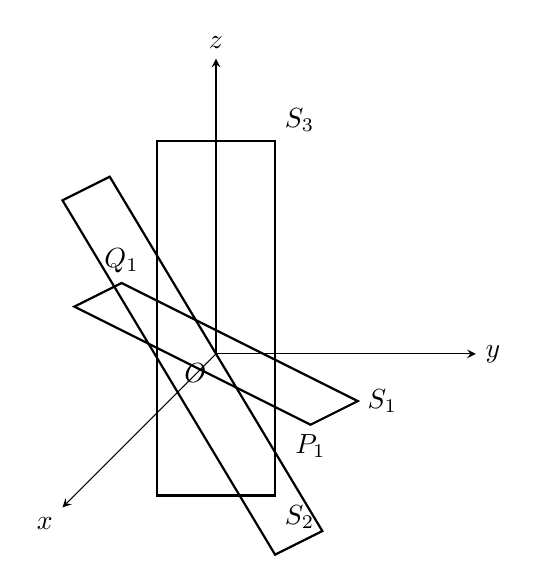
\begin{tikzpicture}[scale=1.5, >=stealth]
    \draw[->] (0,0) -- (-1.3, -1.3) node[below left] {$x$};
    \draw[->] (0,0) -- (2.2, 0) node[right] {$y$};
    \draw[->] (0,0) -- (0, 2.5) node[above] {$z$};
    \node[below left] at (0,0) {$O$};

    \draw[thick] (0.8, -0.6) -- (-1.2, 0.4) -- (-0.8, 0.6) -- (1.2, -0.4) -- cycle;
    \node[below] at (0.8, -0.6) {$P_1$};
    \node[right] at (1.2, -0.4) {$S_1$};
    \node[above] at (-0.8, 0.6) {$Q_1$};

    \draw[thick] (0.5, 1.8) -- (-0.5, 1.8) -- (-0.5, -1.2) -- (0.5, -1.2) -- cycle;
    \node[above right] at (0.5, 1.8) {$S_3$};
    \node[below right] at (0.5, -1.2) {$S_2$};

    \draw[thick] (-0.9, 1.5) -- (0.9, -1.5) -- (0.5, -1.7) -- (-1.3, 1.3) -- cycle;
  \end{tikzpicture}
\end{figure}

\begin{enumerate}
  \item $\triangle P_1P_2P_3$ の面積，および $\triangle P_1P_2P_3$ と原点 $O$ との距離を求めよ．
  \item 四面体 $OP_1P_2P_3$ および四面体 $OP_1P_2S_2$ の体積をそれぞれ求めよ．
  \item $L_1$，$L_2$，$L_3$ の12頂点から3点を選び三角形をつくる．
  このとき $\triangle P_1P_2P_3$ または $\triangle P_1P_2S_2$ と合同な三角形が20個えられる．
  これらの三角形で囲まれる二十面体を $D$ とする．
  $\displaystyle 0<\theta<\frac{\pi}{4}$ なる $\theta$ に対して
  \begin{align*}
    a=\cos\theta, \hspace{1\zw} b=\sin\theta
  \end{align*}
  とおくとき $D$ の体積 $V$ を $t=\tan\theta$ の関数 $V(t)$ として表せ．
  \item $0<t<1$ において $V(t)$ は最大値をとることを示し，そのとき $t$ の値を求めよ．
\end{enumerate}

\end{document}
